\documentclass{standalone}
%
\usepackage{tikz}
\usetikzlibrary{backgrounds,shapes.callouts}
\usepackage{tkz-euclide}
\usepackage{xcolor}
\usepackage{ifthen}
%
\definecolor{space}{HTML}{1F2C4E}
\definecolor{earth}{HTML}{0089FA}
\definecolor{dida}{HTML}{FFDE00}
\definecolor{title}{HTML}{FBA706}
\definecolor{moon}{HTML}{AFAFAF}
%
\usepackage{fontspec}
\setmainfont{Open Dyslexic}
%
\title{La placca del Pioneer}
\begin{document}
	\tikzset{
		partial ellipse/.style args = {#1:#2:#3}{insert path={+ (#1:#3) arc (#1:#2:#3)}},
		notice/.style  = { draw, ellipse callout, callout relative pointer={#1} },
	}
	\begin{tikzpicture}[background rectangle/.style={fill=white},show background rectangle,>={[inset=0,angle'=27]Stealth}]
		%title
		\draw [black,ultra thick,fill=title] (0,9.8) rectangle (30,16.8);
		\node at (15,14.8) {\textcolor{black}{\fontsize{90}{91}\selectfont Il messaggio}};
		\node at (15,11.8) {\textcolor{black}{\fontsize{90}{91}\selectfont del pioniere}};
		%
		\begin{scope}[shift={(0,7)}]
			\draw [ultra thick, fill=dida] (2.5,1.5) rectangle (28,-1.5);
			\node (example-textwidth-2) [right, align=left, text width=25cm, color=black, font=\fontsize{18pt}{19pt}\selectfont] at (3,0) {La missione \emph{Mariner} 9 venne lanciata il 30 maggio del 1971 e si immise in orbita il 14 novembre del 1971. Uno dei giornalisti che seguì la missione fu \textbf{Eric Burgess}.};
		\end{scope}
		%
		\begin{scope}[shift={(0,-1)}]
			%\draw [ultra thick, fill=earth] (20.5,4) rectangle (25.5,-4);
			\node at (23,0) {
\includegraphics[width=5cm]{carl_sagan}};
			\node (example-textwidth-2) [notice={(3,0.5)}, ultra thick, right, align=center, text width=12cm, color=black, fill=white, font=\fontsize{23pt}{24pt}\selectfont] at (1,-1) {Eric si presentò al \emph{Jet Propulsion Laboratory} di Pasadena con un'idea formidabile: mandare un messaggio nello spazio per conto del genere umano a bordo delle sonde \emph{Pioneer}! Andai subito a parlarne con \textbf{Frank Drake}.};
		\end{scope}
		%
		\begin{scope}[shift={(0,-11)}]
			\node at (7,0) {
\includegraphics[width=8cm]{frank_drake}};
			\node (example-textwidth-2) [notice={(-3,0.5)}, ultra thick, right, align=center, text width=12cm, color=black, fill=white, font=\fontsize{23pt}{24pt}\selectfont] at (12,-1) {Carl ottenne dalla NASA il permesso di portare a termine l'idea, a patto di impiegarci non più di tre settimane. Ci mettemmo a tavolino e progettammo il messaggio che poi avrebbe realizzato la moglie di Carl, \textbf{Linda Salzman}.};
		\end{scope}
		%
		\begin{scope}[shift={(0,-21)}]
			%\draw [ultra thick, fill=earth] (20.5,4) rectangle (25.5,-4);
			\node at (23,0) {
\includegraphics[width=8cm]{linda_salzman}};
			\node (example-textwidth-2) [notice={(3,0.5)}, ultra thick, right, align=center, text width=12cm, color=black, fill=white, font=\fontsize{23pt}{24pt}\selectfont] at (1,-1) {All'epoca ero ancora sposata con Carl ed era nato da poco nostro figlio \textbf{Nick}. E penso di essere riuscita a rendere al meglio quello che Frank e Carl avevano in mente.};
		\end{scope}
		%
		\begin{scope}[shift={(0,-51)}]
			%\draw [ultra thick,fill=space] (4,1) rectangle (27,-1);
			%\node (example-textwidth-2) [right, align=center, text width=25cm, color=white, font=\fontsize{23pt}{24pt}\selectfont] at (3,0) {Schema dell'esperimento di Michelson e Morley};
		\end{scope}
		% 
		\begin{scope}[shift={(0,-41)}]
			%\draw [fill=moon] (0,0) circle (10cm);
			\draw [ultra thick, fill=earth!50!white] (8,5.5) rectangle (14,8);
			\draw [ultra thick,->] (14,8) -- (16,10);
			\draw [ultra thick, fill=earth!50!white] (2.5,10) rectangle (28,14);
			\node (example-textwidth-2) [right, align=left, text width=25cm, color=black, font=\fontsize{18pt}{19pt}\selectfont] at (3,12) {Transizione iperfine per inversione di spin dell'atomo di idrogeno, il più abbondante dell'universo. L'inversione dallo spin su a quello giù, e viceversa, permette di descrivere due unità di misura, una di lunghezza, 21 cm, e una di tempo, la frequenza di 1420 MHz, ovvero il periodo di 0.7 ns.};
			%
			\draw [ultra thick, fill=red!50!white] (15,6) rectangle (24.5,-4);
			\draw [ultra thick, ->] (22.5,-4) -- (22.5,-20);
			\draw [ultra thick, fill=red!50!white] (2.5,-20) rectangle (28,-22);
			\node (example-textwidth-2) [right, align=left, text width=25cm, color=black, font=\fontsize{18pt}{19pt}\selectfont] at (3,-21) {Le figure degli esseri umani messe a confronto con quelle del \emph{Pioneer}. Le altezze medie sono ricavabili a partire dai segni posti a sinistra.};
			% freccia per dida Sistema Solare
			\draw [ultra thick, ->] (14,-7.5) -- (14,-16);
			%
			\draw [ultra thick, fill=dida] (9,2.5) rectangle (13,-1.5);
			\draw [ultra thick, ->] (11,-1.5) -- (11,-10);
			\draw [ultra thick, fill=dida] (2.5,-10) rectangle (28,-14);
			\node (example-textwidth-2) [right, align=left, text width=25cm, color=black, font=\fontsize{18pt}{19pt}\selectfont] at (3,-12) {Posizione relativa del Sole rispetto al centro della galassia. Sono poi indicate 14 pulsar con i rispettivi periodi. Il numero di pulsar risulta ridondante, ma necessario poiché non tutte sono visibili da posizioni diverse rispetto al Sistema Solare.};
			%
			\draw [ultra thick, fill=moon!50!white] (5,-3.5) rectangle (21,-7.5);
			%
			\draw [ultra thick, fill=moon!50!white] (2.5,-16) rectangle (18.5,-18);
			\node (example-textwidth-2) [right, align=left, text width=25cm, color=black, font=\fontsize{18pt}{19pt}\selectfont] at (3,-17) {Il Sistema Solare e la traiettoria del \emph{Pioneer}.};			
			%
			\node at (15,0) {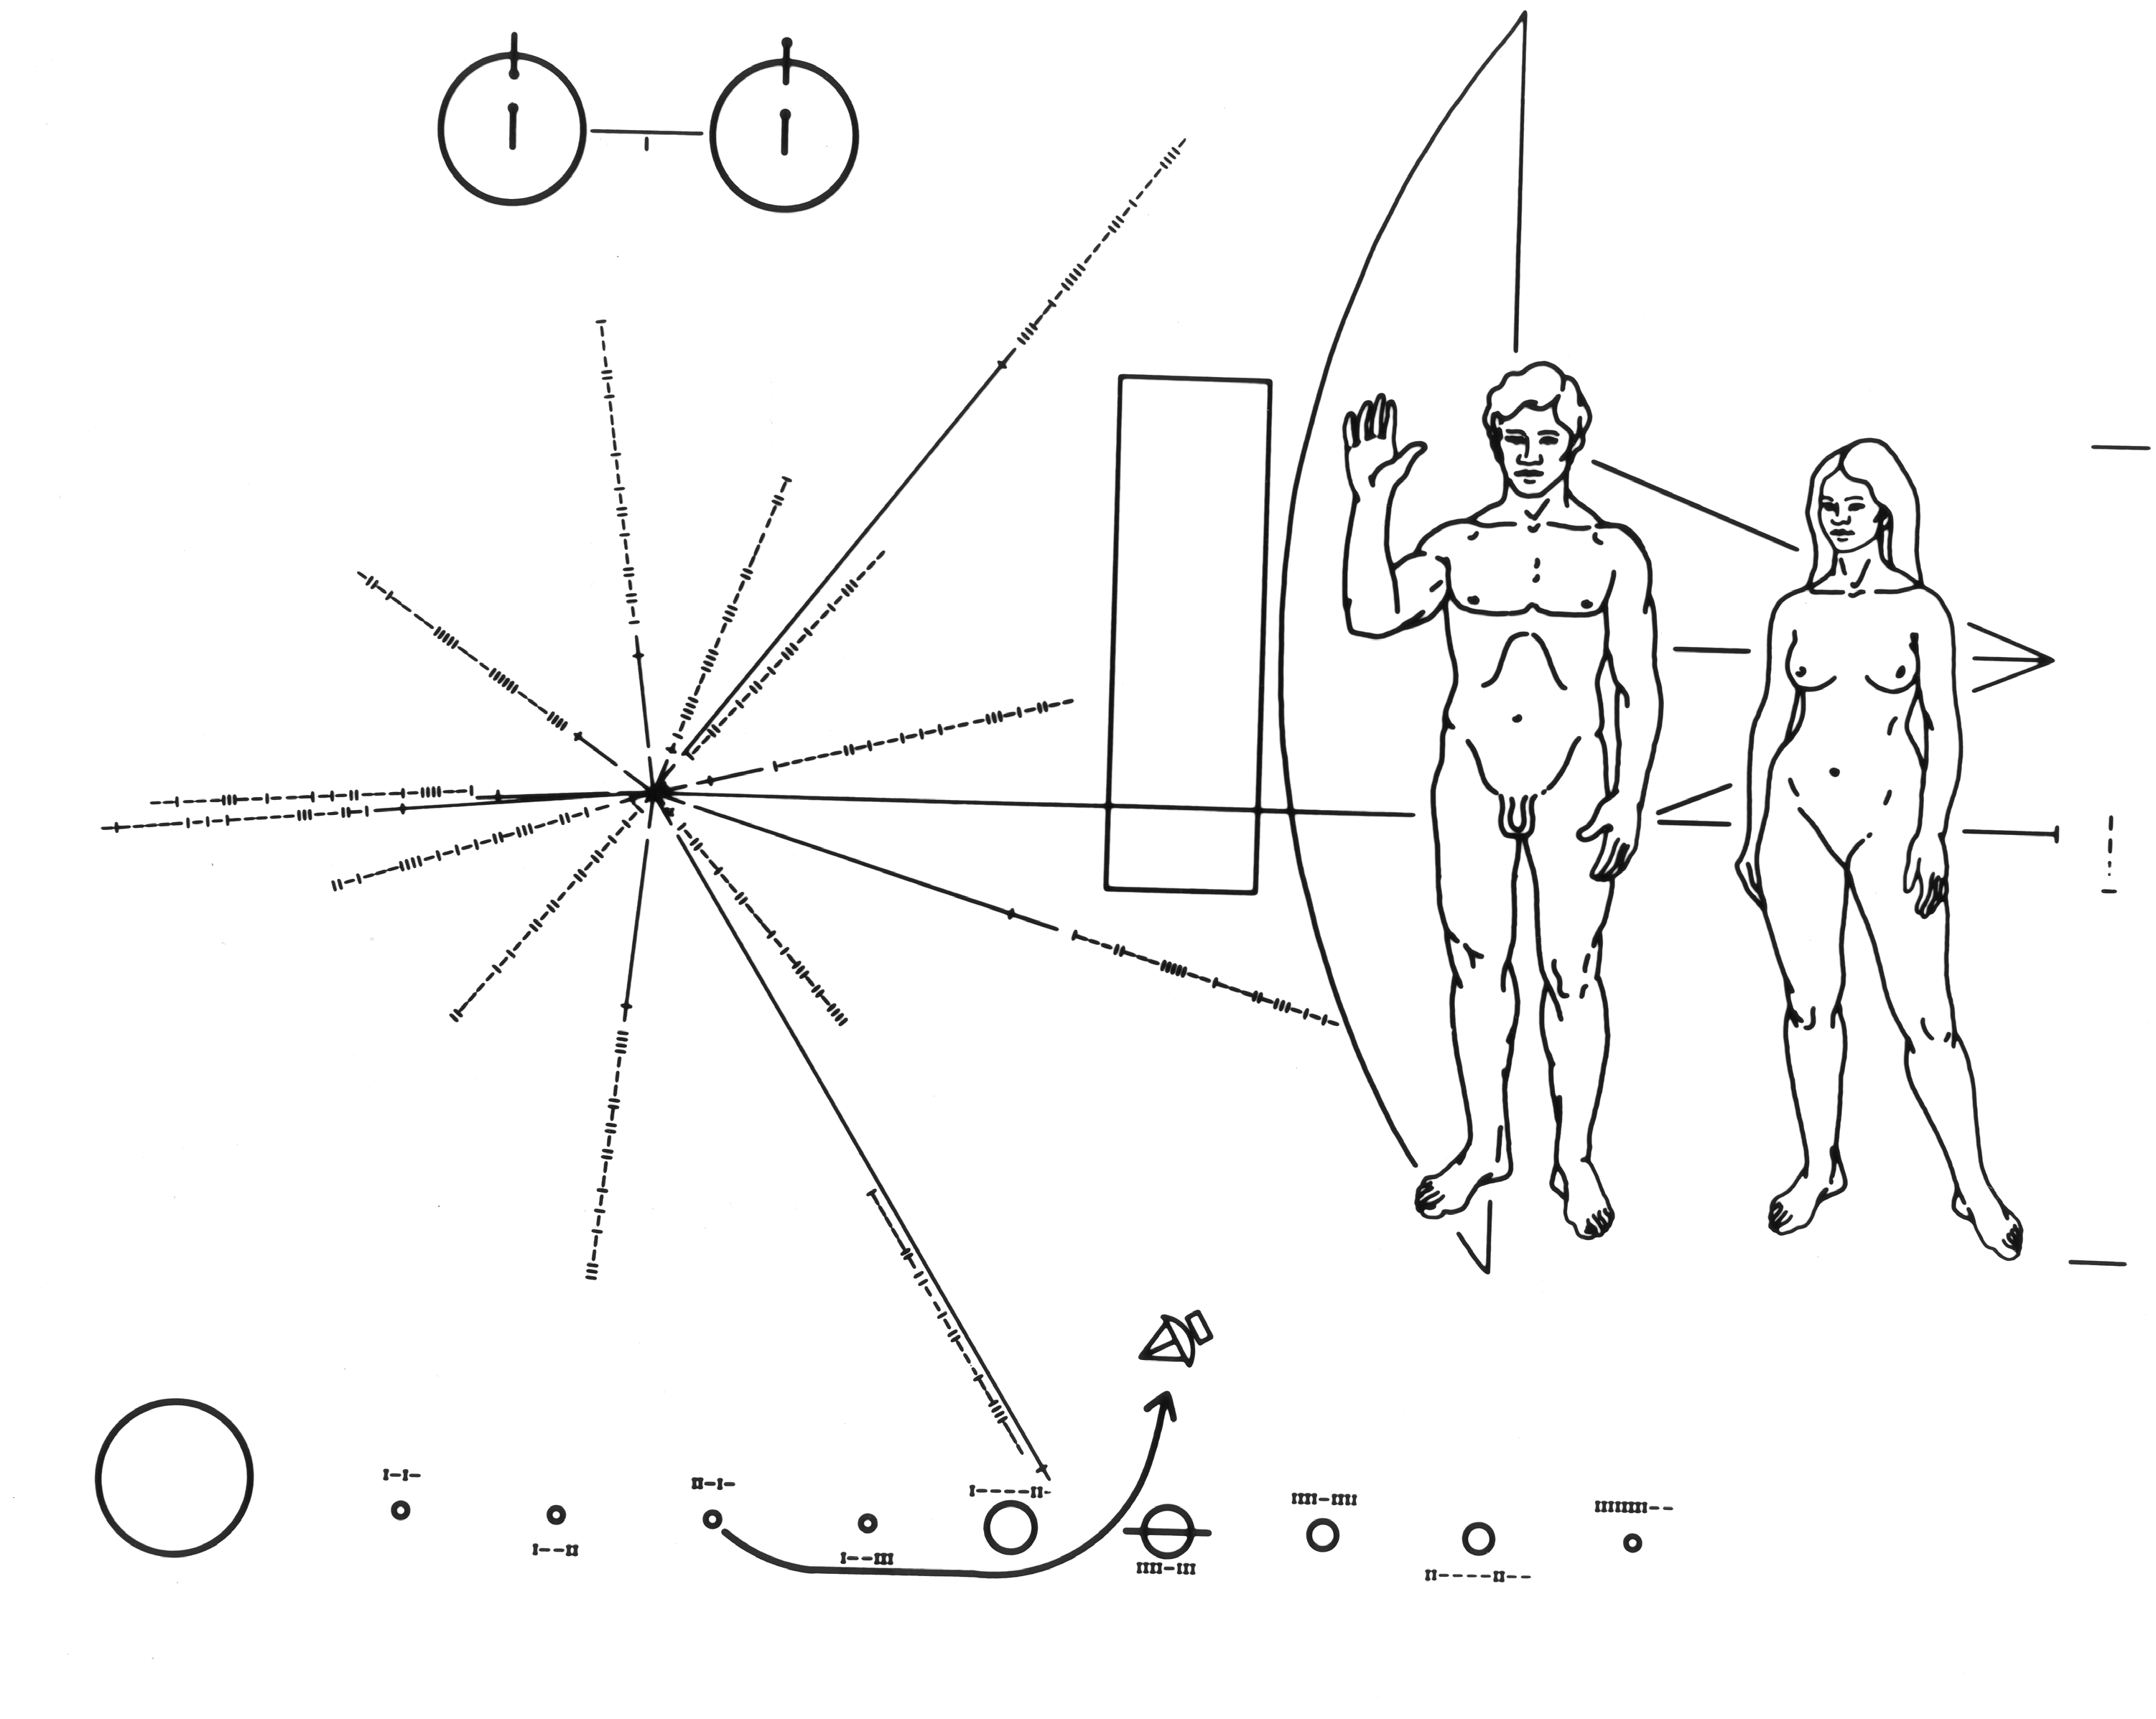
\includegraphics[width=20cm]{pioneer_message}};
		\end{scope}
		%
		\begin{scope}[shift={(0,-66)}]
			\draw [ultra thick, fill=space] (2.5,1.5) rectangle (28,-1.5);
			\node (example-textwidth-2) [right, align=left, text width=25cm, color=white, font=\fontsize{18pt}{19pt}\selectfont] at (3,0) {Vennero realizzate due placche. La prima fu lanciata a bordo del \emph{Pioneer} 10 il 2 marzo del 1972 e la seconda sulla \emph{Pioneer} 11 il 6 aprile del 1973.};
		\end{scope}
		%
		\begin{scope}[shift={(0,-70)}]
			\node at (27,0) () {
\includegraphics[width=3.7cm]{licenza}};
			\node at (15.5,-0.1) {\textcolor{black}{\fontsize{14}{15}\selectfont Testo e illustrazioni, esclusa la placca: @ulaulaman - Gianluigi Filippelli}};
		\end{scope}
	\end{tikzpicture}
%
\end{document}
